\section{Estudio de las Comunidades}

\begin{figure}
  \centering  
  \begin{subfigure}[t]{0.48\textwidth}
    \centering
    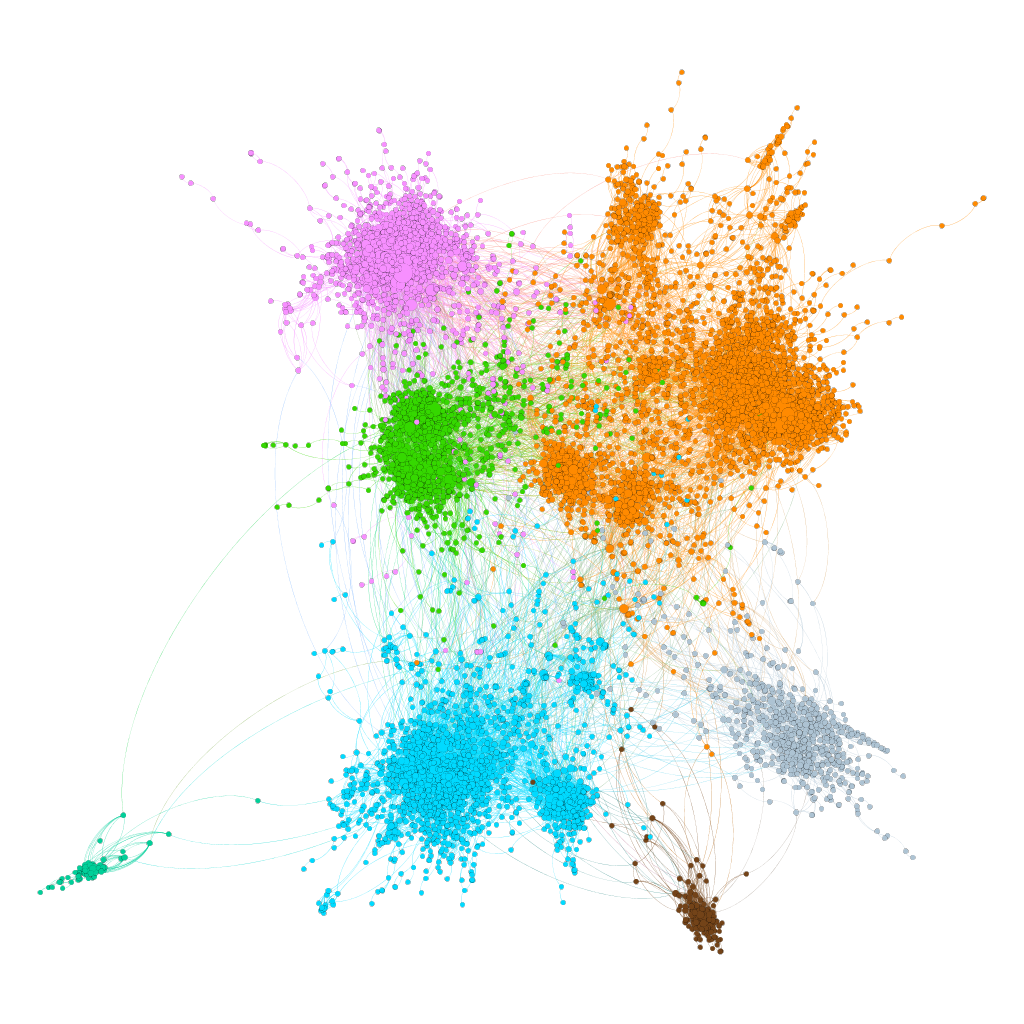
\includegraphics[width=\textwidth]{img/resultados/grado-leinen0.1.png}
    \caption{Coeficiente 0.1.}
  \end{subfigure}
  \vspace{7mm}
  \hfill
  \begin{subfigure}[t]{0.48\textwidth}
    \centering
    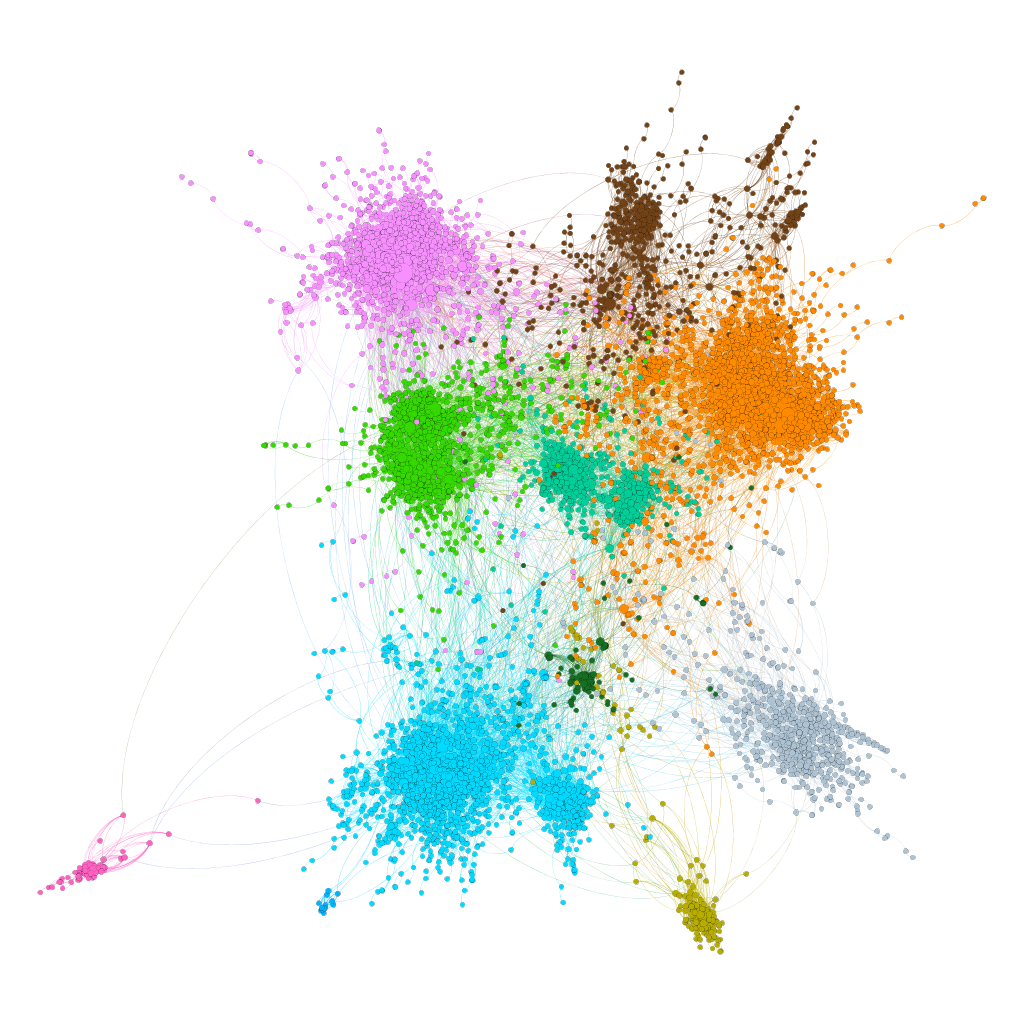
\includegraphics[width=\textwidth]{img/resultados/grado-leinen0.25.png}
    \caption{Coeficiente 0.25.}
  \end{subfigure}
  \hfill
  \begin{subfigure}[t]{0.48\textwidth}
    \centering
    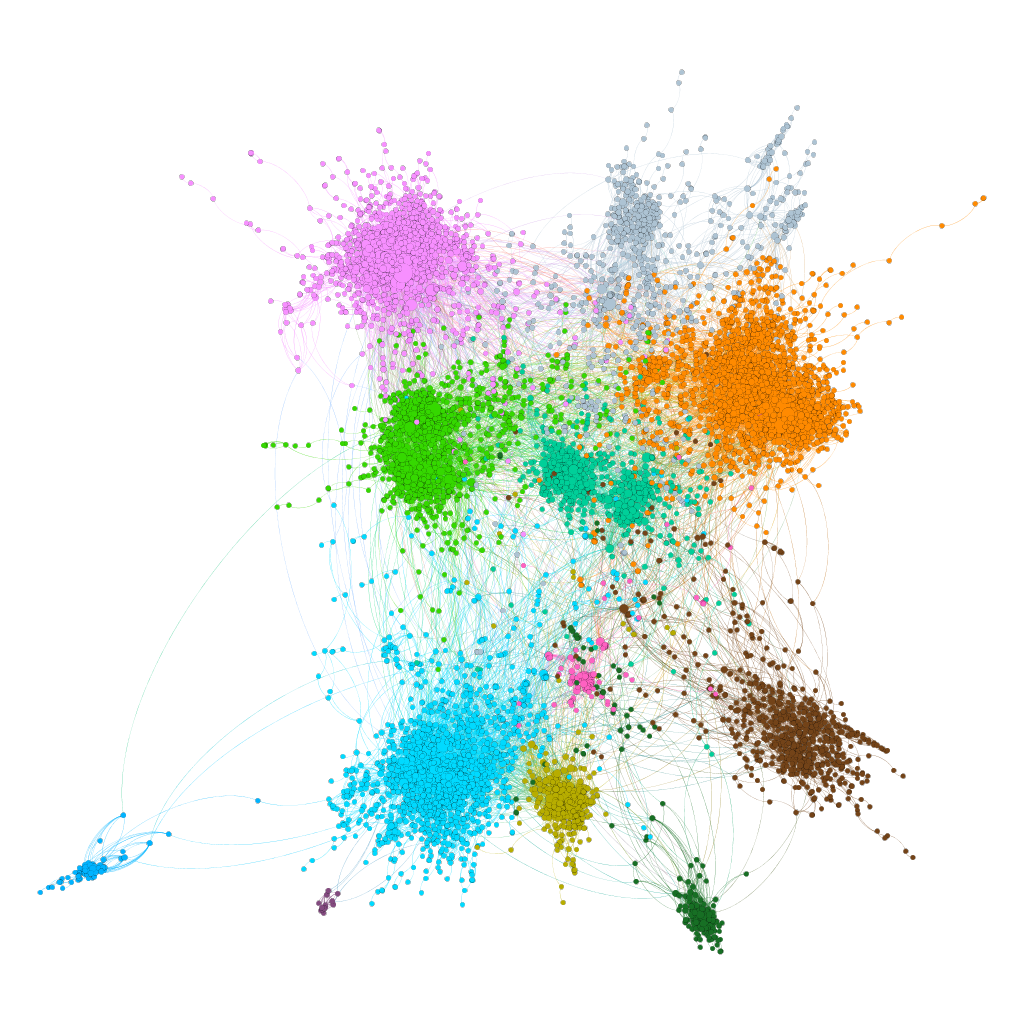
\includegraphics[width=\textwidth]{img/resultados/grado-leinen0.33.png}
    \caption{Coeficiente 0.33.}
  \end{subfigure}
  \hfill
  \begin{subfigure}[t]{0.48\textwidth}
    \centering
    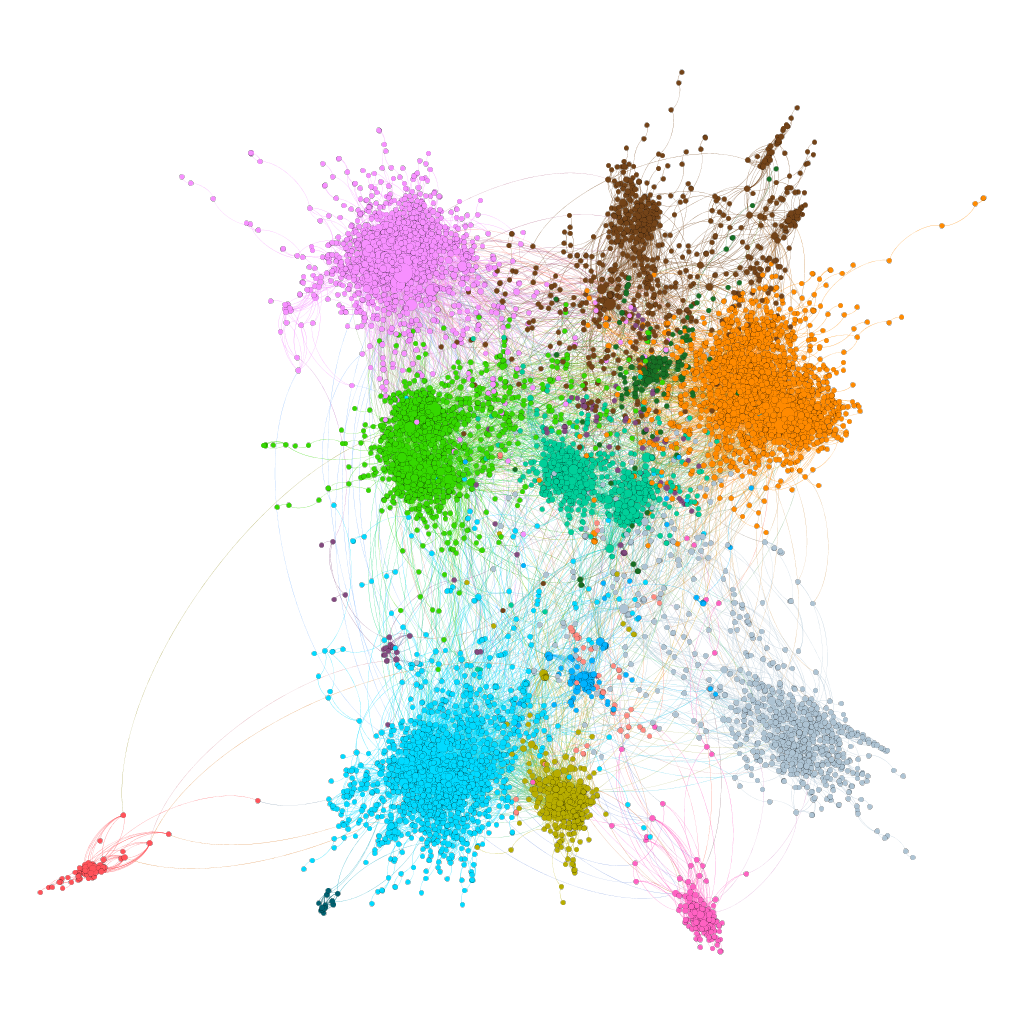
\includegraphics[width=\textwidth]{img/resultados/grado-leinen0.5.png}
    \caption{Coeficiente 0.5.}
  \end{subfigure}

  \caption{Comunidades detectadas por el algoritmo Leinen para diferentes coeficientes.}
\end{figure}

\begin{figure}
    \centering  
    \begin{subfigure}[t]{0.48\textwidth}
      \centering
      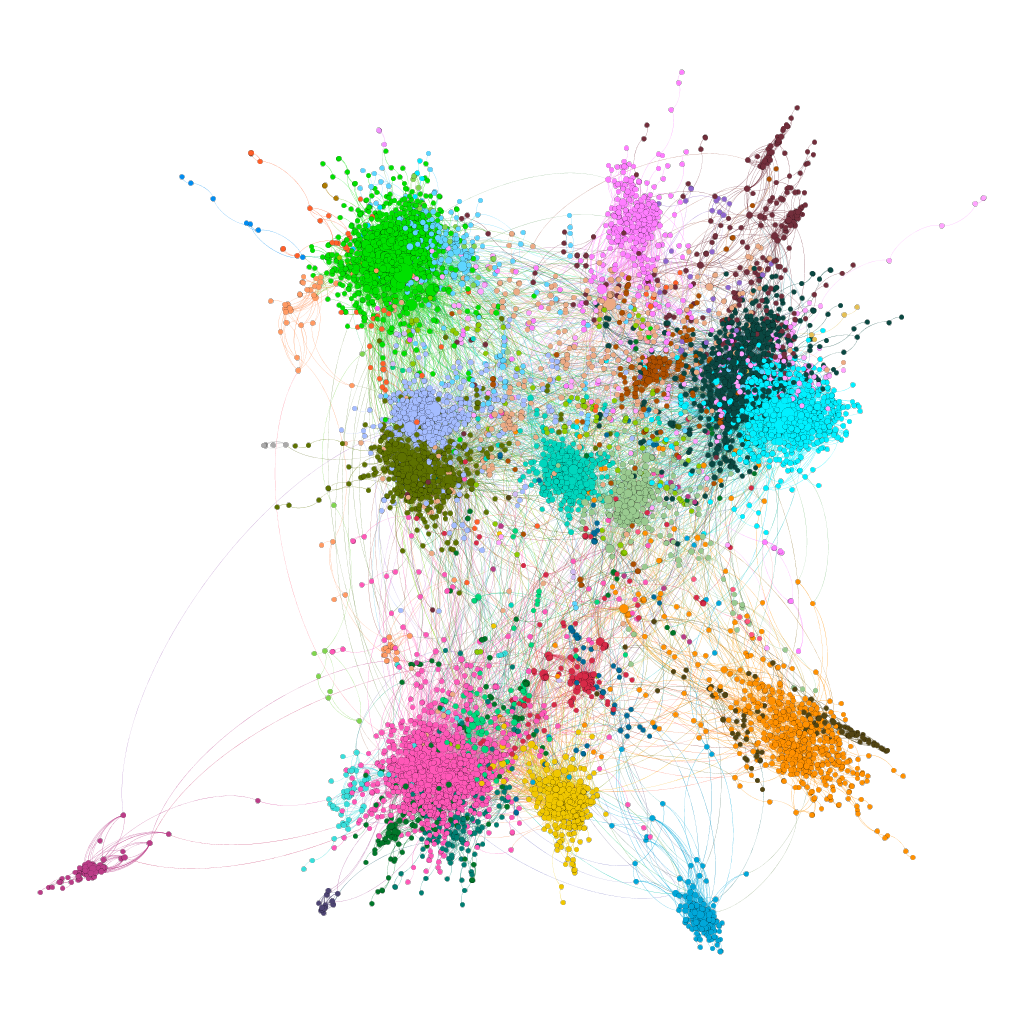
\includegraphics[width=\textwidth]{img/resultados/grado-lovaina0.5.png}
      \caption{Coeficiente 0.5.}
    \end{subfigure}
    \vspace{7mm}
    \hfill
    \begin{subfigure}[t]{0.48\textwidth}
      \centering
      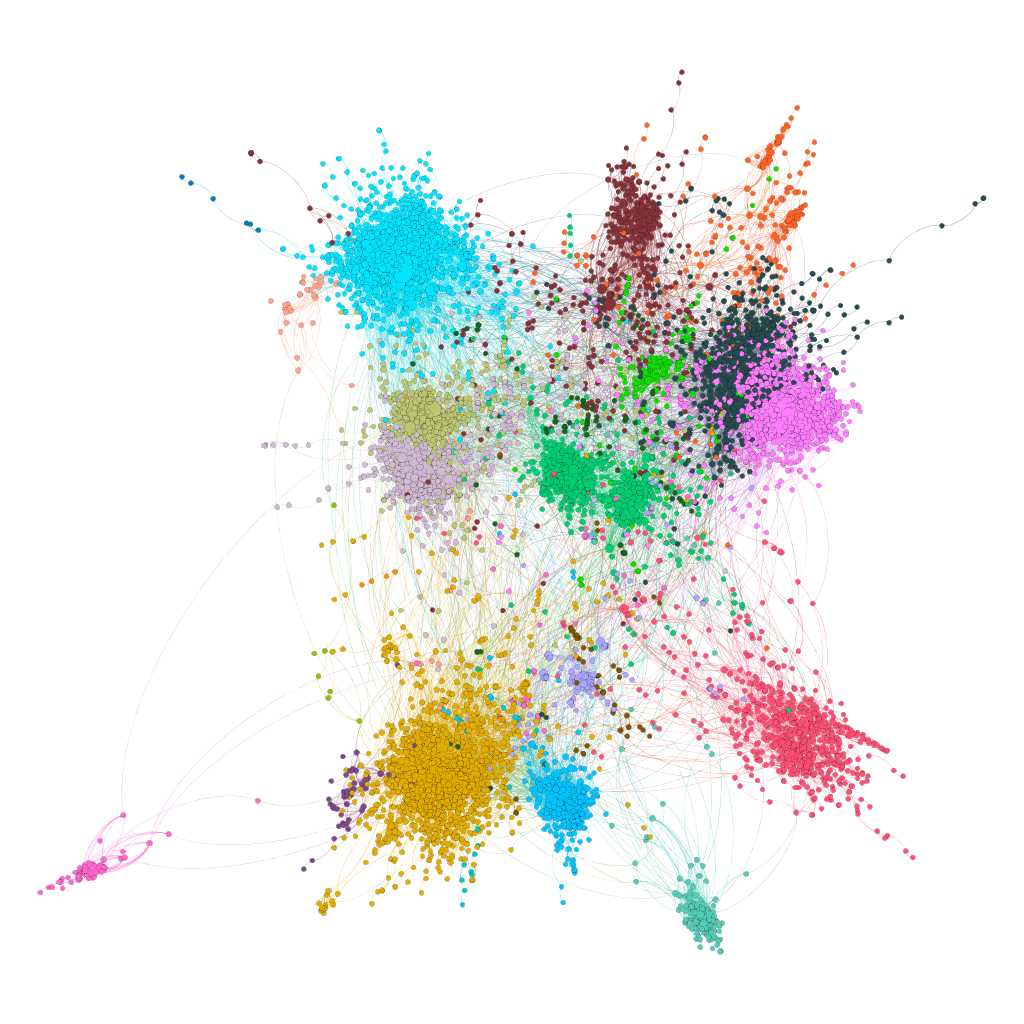
\includegraphics[width=\textwidth]{img/resultados/grado-lovaina1.png}
      \caption{Coeficiente 1.}
    \end{subfigure}
    \hfill
    \begin{subfigure}[t]{0.48\textwidth}
      \centering
      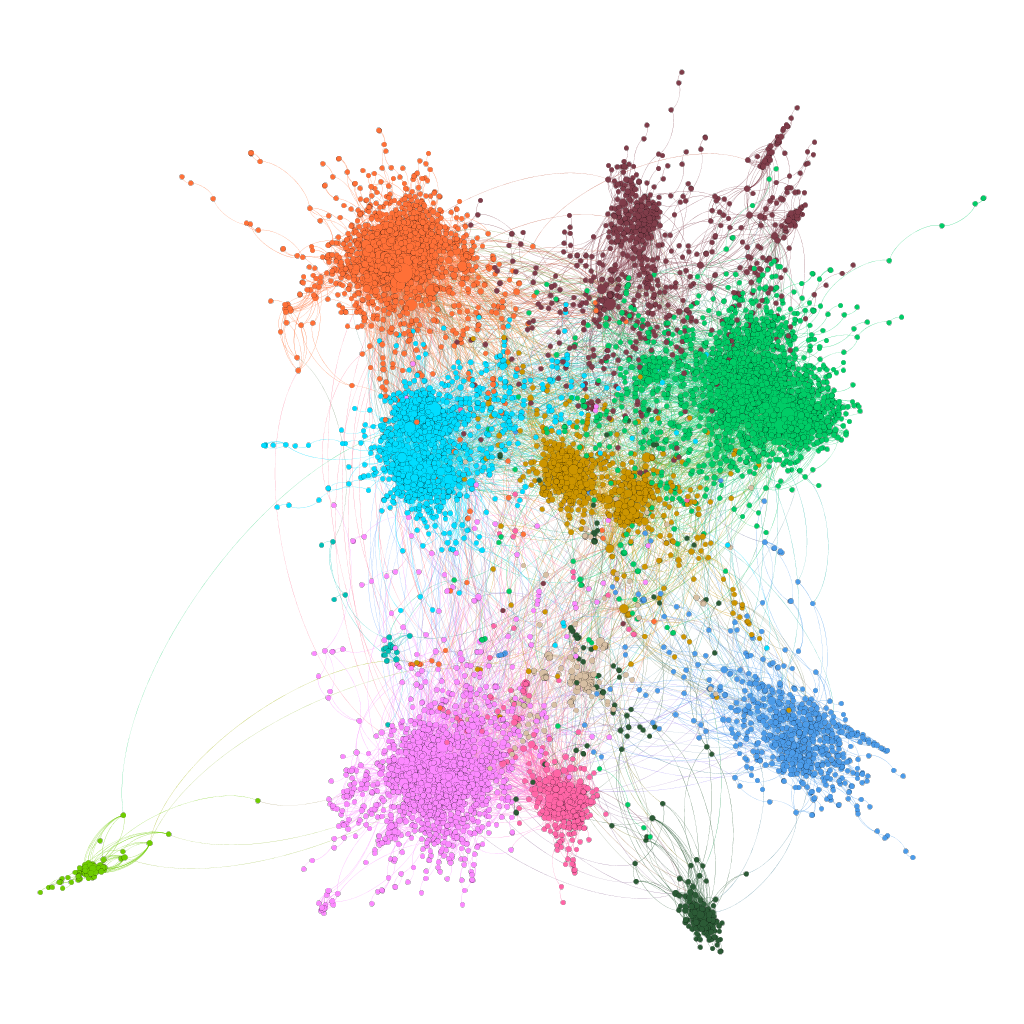
\includegraphics[width=\textwidth]{img/resultados/grado-lovaina2.png}
      \caption{Coeficiente 2.}
    \end{subfigure}
    \hfill
    \begin{subfigure}[t]{0.48\textwidth}
      \centering
      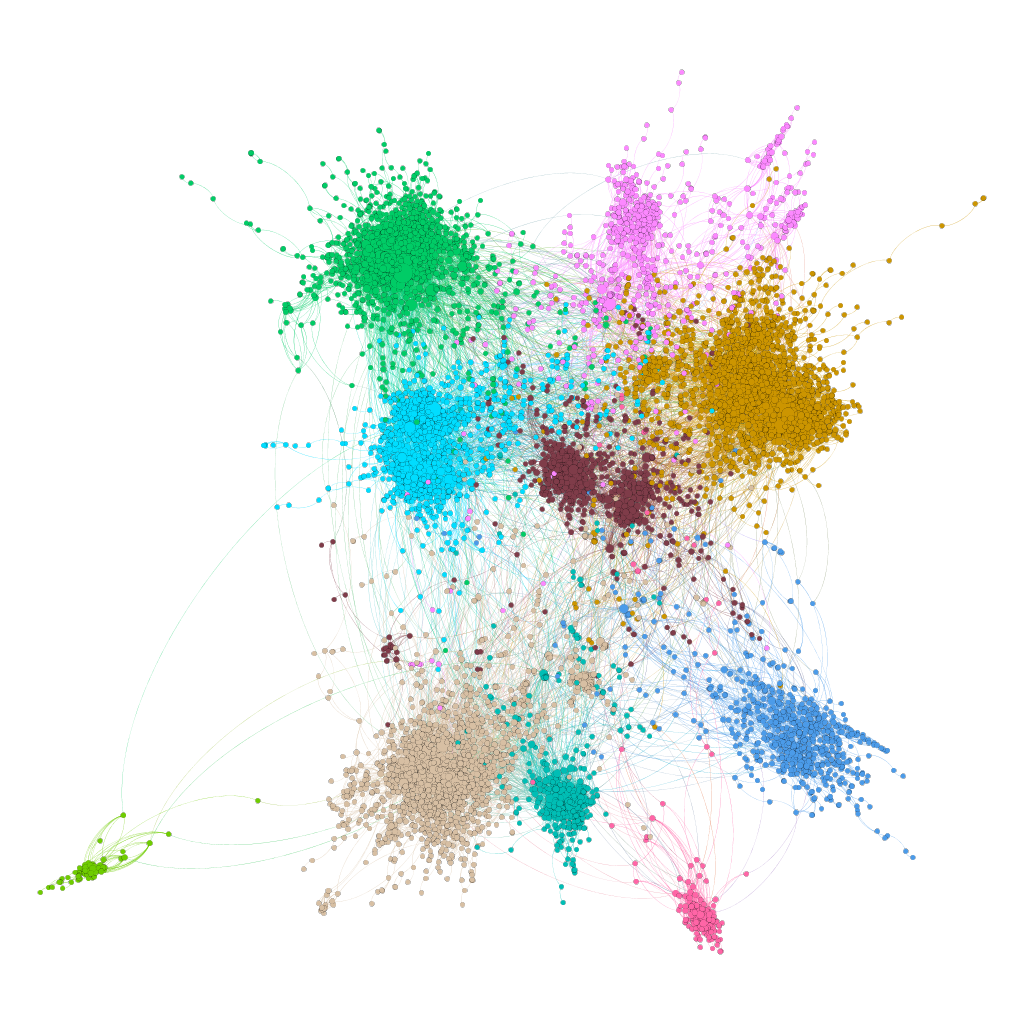
\includegraphics[width=\textwidth]{img/resultados/grado-lovaina3.png}
      \caption{Coeficiente 3.}
    \end{subfigure}
  
    \caption{Comunidades detectadas por el algoritmo Lovaina para diferentes coeficientes.}
\end{figure}

\begin{figure}
  \centering  
  \begin{subfigure}[t]{0.48\textwidth}
    \centering
    \includegraphics[width=\textwidth]{img/resultados/lovaina0.5/communities-size-distribution.png}
    \caption{Coeficiente 0.5.}
  \end{subfigure}
  \vspace{7mm}
  \hfill
  \begin{subfigure}[t]{0.48\textwidth}
    \centering
    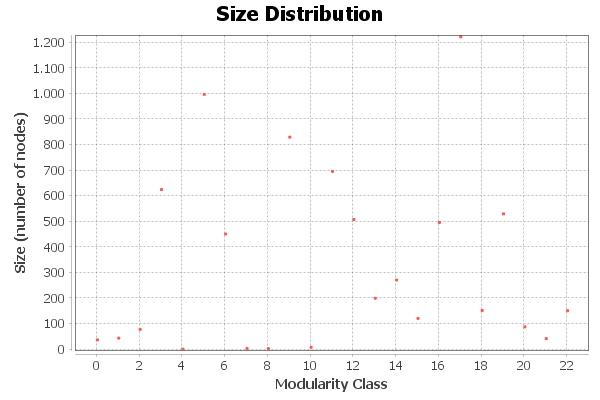
\includegraphics[width=\textwidth]{img/resultados/lovaina1/communities-size-distribution.png}
    \caption{Coeficiente 1.}
  \end{subfigure}
  \hfill
  \begin{subfigure}[t]{0.48\textwidth}
    \centering
    \includegraphics[width=\textwidth]{img/resultados/lovaina2/communities-size-distribution.png}
    \caption{Coeficiente 2.}
  \end{subfigure}
  \hfill
  \begin{subfigure}[t]{0.48\textwidth}
    \centering
    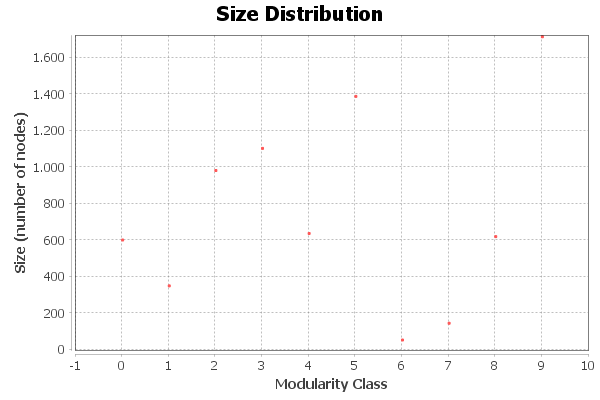
\includegraphics[width=\textwidth]{img/resultados/lovaina3/communities-size-distribution.png}
    \caption{Coeficiente 3.}
  \end{subfigure}

  \caption{Gráfico de distribuciones para el algoritmo Lovaina en diferentes coeficientes.}
\end{figure}

\vspace{2\baselineskip}

\begin{figure}[H]
  \centering
  \resizebox{0.75\columnwidth}{!}{%
  \begin{tabular}{| l | c || c | c |} 
      \hline
      \textbf{Algoritmo} & \textbf{Coeficiente} & \textbf{Modularidad} & \textbf{Clústers}  \\
      \Xhline{2\arrayrulewidth}
      \multirow{4}{*}{Leinen} 
        & 0.1 & 0.941 & 7 \\ \cline{2-4}
        & 0.25 & 0.913 & 11 \\ \cline{2-4}
        & 0.33 & 0.901 & 11 \\ \cline{2-4}
        & 0.5 & 0.878 & 15 \\ \cline{2-4}
      \hline
      \multirow{4}{*}{Lovaina} 
        & 0.5 & 0.800 & 42 \\ \cline{2-4}
        & 1 & 0.813 & 23 \\ \cline{2-4}
        & 2 & 0.806 & 12 \\ \cline{2-4}
        & 3 & 0.803 & 10 \\ \cline{2-4}
      \hline
  \end{tabular}
  }
  \caption{Modularidad y número de clústers obtenido por cada algoritmo.}
\end{figure}

\newpage

La referencia sobre los países puede ser un buen comienzo de partida para la búsqueda de buenas comunidades, pero es importante no dejarse engañar por esto pues existen hubs de diferentes regiones altamente conectados entre sí. Además, algunas de las fronteras entre los hubs de los países son difusas y existen zonas de baja conectividad fuertemente entremezcladas.

El objetivo de la búsqueda de comunidades es después de todo encontrar grupos de usuarios con intereses comunes que nos permitan simplificar el manejo de la red y la transmisión de información. La ubicación regional probablemente sea relevante en la semántica de nuestra red pero no debe ser el factor decisivo para una selección correcta de comunidades.

\vspace{\baselineskip}

A partir de la estructura de la red vemos que la zona central y superior del grafo no muestra una estructura modular clara. Por el contrario, la zona inferior muestra más claramente una partición en un mínimo de cuatro o cinco comunidades, y esto es detectado perfectamente por el método Leinen independientemente del coeficiente, pero no tanto por Lovaina, donde es necesario empujar el coeficiente hacia arriba para separar mejor estos hubs.

\vspace{\baselineskip}

En cuanto a los efectos en la modularidad y el número de clústers que muestra la Figura 18, nos fijamos en que la calidad de las particiones con Lovaina no varía de manera substancial, aunque sí lo hace el número de clústers que forma.

\vspace{\baselineskip}

Sobre las comunidades en sí, visualmente concluímos que un número de diez parece adecuado para esta red, tal y como se consigue en la Figura 16.d. De esta forma contaríamos con cinco clústers bien diferenciados en la parte inferior conectándose a un núcleo central a su vez dividido en cuatro. Este núcleo contaría con la mayoría de nodos de la red fuertemente interconectados entre sí. Por último, nos quedaría un hub denso en la parte superior izquierda con muchas conexiones al núcleo grande.

\vspace{\baselineskip}

En referencia al significado semántico de estas comunidades, es de esperar que los usuarios se agrupen por estilos y géneros de música favoritos donde los intercambios de información vayan sobre esos temas. 

Con una partición en diez podríamos suponer que en el núcleo central predominan los géneros de moda en la cultura asiática actual (la red se construyó en 2020), como es el K-Pop, el J-Pop y el C-Pop, y que en las comunidades inferiores predominan estilos relacionados con estos géneros pero de ámbito menos popular, como el rock, el rap o el pop anglosajón.

Por último, tendríamos un hub interesante en la esquina inferior izquierda, conectándose al resto de la red por muy pocos nodos. Este hub nos podría dar información sobre los géneros menos relevantes en la comunidad, como podría ser el metal, el jazz, o la electrónica.